\documentclass[12pt,a4paper,oneside]{article}
\usepackage[spanish,activeacute]{babel}
\usepackage[utf8]{inputenc}
\usepackage[left = 2.5cm, top = 2cm, right = 2.5cm, bottom = 2cm]{geometry}
\usepackage{amssymb}
\usepackage{graphicx}

\renewcommand{\spanishfigurename}{Figure} %Figura -> Figure

\setcounter{secnumdepth}{3}
\setcounter{tocdepth}{3}

\hyphenation{functions func-tions}

\renewcommand{\baselinestretch}{1}

\newpage\pagenumbering{arabic}
\setcounter{page}{1}

\begin{document}

\newenvironment{itemize*}
        {\begin{itemize}
            \setlength{\itemsep}{1pt}
            \setlength{\parsep}{3pt}
            \setlength{\parskip}{3pt}}
        {\end{itemize}}

\newenvironment{enumerate*}
        {\begin{enumerate}
            \setlength{\itemsep}{1pt}
            \setlength{\parsep}{3pt}
            \setlength{\parskip}{3pt}}
        {\end{enumerate}}


\part*{Abstract}

\section*{Introduction}
The analysis of the evolution of a variable over time lead us to a set of unique problems in statistical inference and modeling: time series analysis. A time series is a sequence of random variables $Y_1,Y_2,Y_3...$  where $Y_t$ denotes the value taken by the time series at time $t$. Generally in time series the values of $t$ are discrete which means that $t \in \mathbb{N}$.

These random variables will generally be temporally correlated, so specific modeling and inference techniques are often needed. The application of these techniques is possible thanks to the computing power currently available, although we must never leave aside the mathematical and statistical theory on which they are based.

There are many different approaches that we can apply to time series. We can opt for a classical or deterministic approach in which we assume that the time series is composed by the combination of several components, each of which represents certain characteristics of the time series. Then the objective is to estimate and combine these components in order to know the behavior of the time series. We can also work with the Box-Jenkins method, which assumes that the time series is the realization of a determined stochastic process, which means that it can be modelled. To achieve this, it uses ARIMA models, which predict future values through a linear function of past values and innovations (residuals) of the time series. In addition, there are other more general techniques based on more complex algorithms, such as neural networks, that allows us to predict future values accurately.

Some of these techniques can be easily implemented through statistical software such as SPSS, Gretl, Stata or even Excel. However, it seems that, currently, some programming languages like $\textsf{R}$, Python or Octave are being used more than before. This is mainly due to three reasons:

\begin{itemize*}
  \item[$\bullet$]They are free software.
  \item[$\bullet$]They rely on mass collaboration so it is possible to find the latest statistical techniques implemented with immediacy.
  \item[$\bullet$]They offer many possibilities for development because we can modify the code of the different techniques.
\end{itemize*}

Of all the mentioned languages the most used within the statistical community is $\textsf{R}$, since it is completely focused on data analysis. It has a large number of packages available with functions that implement techniques for the preprocessing and prediction of time series.

Despite all the advantages said, many professionals and researches give up the possibilities offered by these programming languages because learning this kind of languages is not easy and requires a great investment of time. From this arises the interest of elaborating a guide or manual that allows the user to extract value of its time series with the programming language $\textsf{R}$. For this it is necessary to know the theory behind the most used techniques as well as its correct implementation. Due to this, an exhaustive bibliographical research of the statistical theory and the $\textsf{R}$ packages needed has been carried out.

As a result, we have been able to develop a guide that we hope will be useful to those professionals and researchers who need to carry out an exhaustive analysis of time series. In order to this, we make a tour through time series processing cycle with the language $\textsf{R}$: data structuring, preprocessing, modeling, model checking and prediction. In addition, different packages are compared in terms of predictive capacity and efficiency.

\section*{Objectives}
The main objectives of this work are:

\begin{itemize*}
  \item[$\bullet$]Carry out a bibliographical research of the most used packages in $\textsf{R}$ focused on time series analysis and the theory behind the techniques applied by them.
  \item[$\bullet$]Provide users with a guide that shows the time series processing cycle in $\textsf{R}$.
\end{itemize*}

The specific objectives of this work are:

\begin{itemize*}
  \item[$\bullet$]Introduce the theory needed to understand time series and some of the most used techniques for its analysis.
  \item[$\bullet$]Study some of the most used packages available in $\textsf{R}$ for data structuring.
  \item[$\bullet$]Study the preprocessing and modeling functions implemented in the $\verb!forecast!$ package.
  \item[$\bullet$]Study the $\verb!TSeries!$ package, emphasizing the implementation of resampling techniques.
  \item[$\bullet$]Study the characteristics of the $\verb!FitARMA!$ package.
  \item[$\bullet$]Study the functions focused on forecast combinations implemented by the $\verb!opera!$ package.
  \item[$\bullet$]Compare the different packages in terms of utility, efficiency and results.
\end{itemize*}

To meet these objectives the work has been structured as follows: first, some general concepts are presented in order to understand the time series and some of the most used techniques. Then we will introduce the $\verb!stats!$, $\verb!zoo!$ and $\verb!xts!$ packages in order to study the different ways that $\textsf{R}$ has to structure this type of data. In addition, some basic functions for the preprocessing of the time series will be studied. Once we have structured our data, we will study the $\verb!forecast!$ package. We will begin with a preprocessing in which we will study the stationarity and we will decompose the time series. We will then go through several models in order of complexity, starting with naive models and ending with the implementation of ARIMA models and neural networks. We will compare the different models respect to their predictive power. We will perform the same process on the $\verb!TSeries!$ package, with special emphasis on resampling techniques. With this package we will also implement several unit root tests. Next, we will study the implementation of the ARMA models that the $\verb!FitARMA!$ package performs, and we will compare its execution time with previously studied packages. With the $\verb!opera!$ package we will combine the predictions made by three different models in order to see if that improve the predictions. Finally, we will compare these packages according to efficiency, utility and predictive power.

\section*{Time series structuring in $\textsf{R}$}
To structure the data it is necessary to use packages that define a class of objects aimed to time series. $\verb!Stats!$ is one of the packages that compose the $\textsf{R}$ base and allows us to define a $\verb!ts!$ object, in addition it implements other useful functions like $\verb!window()!$, which it is used to select subsets of time series.

Another package widely used for this purpose is $\verb!zoo!$ which implements functions to define objects capable of storing time series. This package also includes some functions for applying basic preprocessing techniques aimed at introducing lags or replacing $\verb!NAs!$. Two functions able to apply a moving average ($\verb!rollapply()!$ and $\verb!rollmean()!$) have been compared in terms of computational cost.  For this, we have used the function $\verb!system.time()!$, implemented in the $\textsf{R}$ base.

Another package derived from $\verb!zoo!$ is $\verb!xts!$. In this case the objects are structured in the same way as $\verb!zoo!$, except that we now use the function $\verb!xts!$. Due to the object’s own structure it is possible to convert almost any class of object to $\verb!xts!$ thanks to the $\verb!as.xts()!$ function. It is also explained how to manually select subsets of the time series through the special \textit{subsetting} that it implements.

\section*{Time series modeling}
To study time series modeling in $\textsf{R}$ we will use the data corresponding to the monthly traffic fatalities in Ontario between 1960 and 1974. To compare the predictive power of the different models we will divide the time series into two sets: training and test set. In the first one we train our models whereas in the second we evaluate them.

$\verb!Forecast!$ package is oriented to the preprocessing and analysis of time series. It implements several functions capable of extracting and graphing the different components of the time series, this allow us to be able to study its characteristics better with the objective of fitting the appropriate models. It also includes functions like $\verb!ndiffs()!$ that help us decide on the differencing of the time series.

This package gives us the possibility to fit naive models, in which simple predictions are made, such as $\verb!meanf()!$ that implements a model to predict only with the mean, or $\verb!snaive()!$ that replicates the previous seasonal period. Obviously this type of models do not give us good predictions, this is why we fit more complex models.

Holt-Winters seasonal method is implemented in this package by the $\verb!hw()!$ function and performs an exponential smoothing on several components, then combines them and makes predictions. Several neural network models are also fitted through $\verb!nnetar()!$. These neural networks are constituted by a single hidden layer and take as inputs certain lagged values of the time series. To avoid problems it is important, in this type of models, to control certain parameters, one of them is the regularization parameter. After testing with several configurations we get a model that predicts with very low error.

This package covers all the stages of the Box-Jenkins method. It allows us to perform a data preprocessing through functions such as $\verb!Box.Cox()!$ or $\verb!nsdiffs()!$. It also includes functions like $\verb!Acf()!$ and $\verb!Pacf()!$ that help us identify and select the correct model. To implement ARIMA models, we must use $\verb!Arima()!$. With this function we have fitted several models and compared them respect to several measures (information criteria, predictive power and residual autocorrelation). With this we have seen that the inclusion of a type of constant improves the results. Another very useful function available in this package is $\verb!auto.arima()!$, as it is able to identify and automatically select the model that best fits the data.

Another package oriented to time series analysis is $\verb!TSeries!$. It contains several functions of preprocessing and modeling, although only those responsible for implementing ARMA models will be studied. Its preprocessing is notable for the large number of statistical tests available, some of them test the unit root and others the non-linearity in trend. With these tests we are able to study the time series and guarantee the assumptions necessary to work with ARMA models. Some of the functions that implement these tests are: $\verb!adf.test()!$ that implements Dickey-Fuller test, $\verb!pp.test()!$ that implements Phillips-Perron test or $\verb!terasvirta.test()!$ that contains the non-linearity test of Terasvirta.

One of the strengths of this package is the implementation of different resampling techniques. These techniques are based on bootstrap, with the difference that they manage to maintain the temporal correlation of the time series using a variation known as Moving Block Bootstrap (MBB). This technique is implemented through $\verb!ts.bootstrap()!$ and allows us to generate time series with a temporal structure similar to the original one. With these new time series we can make estimations of the autocorrelation function in order to study its behavior. A similar function also included in the package is $\verb!surrogate()!$. The techniques it implements are based on Fourier transform, and allow us to generate subseries capable of maintaining the temporal structure of the original time series.

We have fitted ARMA models to our data from the $\verb!arma()!$ function. Then we studied the residuals of these models with the Jarque Bera test and the nonparametric BDS test implemented with $\verb!bds.test()!$. The null hypothesis of this test is that the data are independent and identically distributed (i.i.d).

The $\verb!FitARMA!$ package implements ARIMA models based on an algorithm that approximate the maximum likelihood function through an AR of a higher order, this reduces the computational cost of the fit. These models are fitted using the $\verb!FitARMA()!$ function. In order to work with this package we have seasonally adjusted and differenced the time series with functions of the $\verb!forecast!$ package. We have fitted models with different orders and we have done a search on the $\verb!pApprox!$ argument to find the value that optimizes the fit. A simulation has been used to test the efficiency of the functions that implement ARIMA models ($\verb!Arima()!$, $\verb!arma()!$ and $\verb!FitARMA()!$). The results show that $\verb!FitARMA()!$ needs much more time to make the adjustment than $\verb!Arima()!$ and $\verb!arma()!$, and that the last two seem to behave in a similar way.

Finally we used the $\verb!opera!$ package to combine the predictions generated by three different models: neural network, SARIMA and Holt-Winters. By combining these models, we can obtain predictions that fit better the data, since they take into account the results of the three models.

What these techniques do is to weight the predictions of the different models according to their predictive power at a given time $t$. To do this it implements two variations of these techniques: offline combinations and online combinations. The first one is implemented through $\verb!oracle()!$ and allows us to adjust all these weights when we have the whole test set. Through the linear and convex combinations of predictions we have been able to improve the predictive power of individual models.

The online combination is implemented through $\verb!mixture()!$ and it adjusts the weights as new test set values arrive. This function can be very useful when we do not have the whole test set or when we want our predictions to improve over time.

\section*{Conclusions}
The writing of this guide has allowed us to obtain a deeper knowledge about the time series analysis in $\textsf{R}$.

Sometimes, the most laborious part is the data structuring. You have to be very careful when generating the date, because $\textsf{R}$ does not stand out in the treatment of this type of objects. In this case, $\verb!ts!$ class accepts dates without entering $\verb!date!$ class objects, so it can be useful when the time series is structured regularly, however the $\verb!zoo!$ and $\verb!xts!$ classes are recommended when this structure is irregular. The functions oriented to the treatment of $\verb!NAs!$ included in the $\verb!zoo!$ package work very well and are really useful. In addition, if we want to do some simple treatment of the data we can do it with functions like $\verb!rollmean()!$ and $\verb!rollapply()!$. $\verb!Xts!$ package implements a simpler cross-class conversion so it is sometimes better to use $\verb!xts!$ instead of $\verb!zoo!$. If it is needed to do some data preprocessing it is advisable to use $\verb!zoo!$ or $\verb!xts!$ and, at the moment we have the time series ready, we convert it to class $\verb!ts!$, despite its simplicity, it is the one mostly used and it has the least compatibility problems with other packages.

One of the strengths of the $\verb!forecast!$ package is its variety since it includes a large number of functions responsible for implementing different models, most of them focused on prediction. This variety allows us to design a search for the optimal model based on complexity, that is, we can start with simple models and go up in complexity until we find one that, without being excessively complex, offers us the results we are looking for. It also provides functions oriented to the time series preprocessing, being able to difference, decompose, introduce lags, apply unit root tests or study the seasonality without having to use another package. Once a model is fitted, it is easy to predict with it and compare the results with the test set, being able to obtain a large number of accuracy measurements. It also includes very useful functions to study residuals and check for white noise.

$\verb!TSeries!$ package is not as complete as $\verb!forecast!$ but it contains some useful tools. Implements a multitude of statistical tests, which can be very useful to study our time series in order to fit one model or another. It also implements techniques of resampling, something difficult to find in this type of packages. By not including functions oriented to the preprocessing is necessary to use other packages. It only implements ARMA models, so this preprocessing is necessary. Once fitted the model, this package does not give us the option to predict with it, so we would need to write a function that takes care of this, something that can become very laborious.

The $\verb!FitARMA!$ package is similar to $\verb!TSeries!$ with the difference that it is only oriented to fit ARIMA models. It is characterized by the algorithm it uses for estimation. In theory this algorithm makes the function fit the model with a lower computational cost in comparison to other packages, however we have seen that the best timings are obtained with the functions included in $\verb!forecast!$ and $\verb!TSeries!$ packages.

\begin{figure}
    \centering
    \centerline{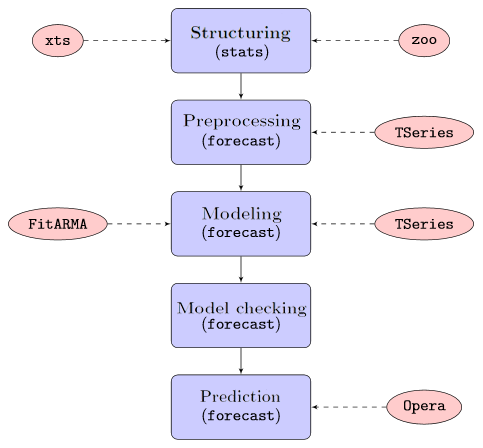
\includegraphics[scale = 0.4]{scheme.png}}
    \caption{Time series processing cycle in $\textsf{R}$}
    \label{esquema}
\end{figure}

$\verb!Opera!$ package allows us to improve predictions by combining several models. It allows us to make these combinations with or without the time factor. In addition, some functions offer very useful graphs that help us to visualize the results. It is a more complicated package to use than the previous ones but can give us very good results.

The time series processing cycle in R developed in this work can be summarized in the following stages, which are also shown in Figure \ref{esquema}.

\begin{itemize*}
  \item[$\bullet$]\textbf{Structuring}: Use the $\verb!zoo!$ and $\verb!xts!$ packages to preprocess the data if necessary. Convert the final object to $\verb!ts!$.
  \item[$\bullet$]\textbf{Preprocessing}: Use the $\verb!forecast!$ package. We can rely on functions from the $\verb!TSeries!$ package.
  \item[$\bullet$]\textbf{Modeling}: With $\verb!forecast!$ should be enough. We can rely on $\verb!TSeries!$ and $\verb!FitARMA!$, although it is not usually necessary.
  \item[$\bullet$]\textbf{Model checking}: $\verb!Forecast!$ has many functions to check the fitted models.
  \item[$\bullet$]\textbf{Prediction}: We obtain the initial predictions with $\verb!forecast!$. If we have fitted more than one model we can improve the results with $\verb!opera!$.
\end{itemize*}

\end{document}
